\documentclass[12pt,a4paper]{article}
\usepackage[utf8]{inputenc}
\usepackage[czech]{babel}
\usepackage[T1]{fontenc}
\setlength{\parskip}{12pt}
\usepackage{fullpage}
\setlength{\parskip}{6pt}
\usepackage{ amssymb }
\usepackage{ mathrsfs }
\usepackage{amsthm}
\usepackage{amsmath}
\usepackage{fixltx2e}
\newtheorem{definition}{Definice}
\newtheorem{sentence}{Věta}
\newtheorem{example}{Příklad}
\newtheorem{result}{Důsledek}
\usepackage{graphicx}
\usepackage{ dsfont }

\begin{document}

\title{Státnicový okruh 1: \\ Matematické metody}
\maketitle
\newpage
\tableofcontents
\newpage
\textbf{Množiny, operace s množinami, kartézský součin množin, konečné, spočetné a nespočetné množiny. Číselné
množiny. Princip indukce. Relace a jejich vlastnosti, operace s relacemi, reprezentace relací. Binární relace na
množině, uzávěry relací, ekvivalence, rozklad na množině, uspořádané množiny. Zobrazení a jejich vlastnosti.}

\section{Množiny}
Množina je objekt, který se skládá z jiných objektů tzv. \textbf{prvků} té množiny. Množiny zpravidla značíme velkými písmeny (A, B, \dots, Z), jejich prvky pak malými písmeny (a, b, \dots, z). Fakt, že $x$ je prvkem množiny $A$ značíme $x \in A$. Není-li prvkem $A$ značíme $x \not\in A$.

Množina je jednoznačné dána svými prvky. Prvek do množiny buď patní nebo ne. Nemá tedy smysl hovořit o pořadí prvků a také nemá smysl zabývat se tím kolikrát se daný prvek v množině nachází.
Speciální množinou je tzv. \textbf{prázdná množina} značíme $\emptyset$. Tato množina neobsahuje žádné prvky tedy pro všechna $x$ platí, že $x \not\in \emptyset$.

\subsection{Dělení množin}
Množiny dělíme na \textbf{konečné} a \textbf{nekonečné}. Množina $A$ se nazývá konečná právě když existuje přirozené číslo $n$ tak že prvky této množiny můžeme očíslovat čísly 1, 2, \dots, $n$. Číslo $n$ nazveme počet prvků množiny a značíme jej $|A|$
Pokud $|A| = \infty$ nazveme množinu nekonečnou a říkáme, že má nekonečně mnoho prvků.

\textbf{Spočetná} množina znamená zjednodušeně řečeno „množina, jejíž prvky lze spočítat“. Spočítáním se zde rozumí očíslování prvků množiny přirozenými čísly - přitom je jedno, zda použiji konečný nebo nekonečný počet přirozených čísel.

\subsection{Zapisování množin}
Množiny můžeme zapisovat následujícími způsoby:
\begin{enumerate}
	\item \textbf{Výčtem prvků} - Množinu která obsahuje prvky $a_1,a_2,\dots,a_n$ zapíšeme následovně $\{a_1,a_2,\dots,a_n\}$.
	\item \textbf{Pomocí charakteristické vlastnosti} - Množina obsahuje právě ty prvky, které splňují vlastnost $\varphi(x)$ zapisujeme $\{x | \varphi(x)\}$. Vlastnost $\varphi(x)$ může být popsána i slovně. Příklad $\varphi(x)$: číslo x je sudé.
\end{enumerate}
\subsection{Vztahy mezi množinami}
Základními vztahy mezi množinami jsou \textbf{rovnost} (=) a \textbf{inkluze} ($\subseteq$)
\begin{itemize}
	\item[] $A = B$ znamená, že pro každé $x : x \in A$ právě když $x \in B$
	\item[] $A \subseteq B$ znamená, že pro každé $x$ : jestliže $x \in A$ pak $x \in B$
	\item[] $A \not= B$ znamená že neplatí $A = B$
	\item[] $A \not\subseteq B$ znamená, že neplatí $A \subseteq B$
\end{itemize}

Množina jejichž prvky jsou právě všechny podmnožiny dané množiny $X$, nazýváme \textbf{potenční množina} množiny $X$ značí se $\mathscr{P}(X)$ nebo také $2^X$. Tedy $2^X = \{A|A\subseteq X\}$.

\subsection{Operace s množinami}
Mezi základní operace s množinami patří průnik (značí se $\cap$), sjednocení (značí se $\cup$), rozdíl (značí se $\setminus$).

Jsou-li $A,B$ množiny, definujeme množiny $A \cup B, A \cap B, A \setminus B$ následovně:
\begin{itemize}
	\item[] $A \cap B = \{ x|x \in A \text{ a } x \in B\}$
	\item[] $A \cup B = \{ x|x \in A \text{ nebo } x \in B\}$
	\item[] $A \setminus B = \{ x|x \in A \text{ a } x \not\in B\}$
\end{itemize}

Množiny nazýváme navzájem disjunktní právě když $A \cap B = \emptyset$.

\subsubsection{Vlastnosti operací}
\begin{itemize}
	\item $A \cap \emptyset = \emptyset, \hspace{10pt} A \cup \emptyset = A,\hspace{10pt} A \cap A = A$
	\item $A \cup B = B \cup A, \hspace{10pt} A \cap B = B \cap A$
	\item $(A \cup B) \cup C = A \cup (B \cup C)$
	\item $A \cap (B \cup C) = (A \cap B) \cup (A \cap C), \hspace{10pt} A \cup (B \cap C) = (A \cup B) \cap (A \cup C)$
	\item $A \cup (A \cap B) = A, \hspace{10pt} A \cap (A \cup B) = A$
\end{itemize}

\section{Princip indukce}
Princip matematické indukce umožňuje dokazovat tvrzení ve tvaru \uv{pro každé přirozené číslo $n$ platí $V(n)$}, kde $V(n)$ je nějaké tvrzení, které závisí na $n$ (např. $1 + 2 + \dots + n = \frac{n(n+1)}{2}$).

\begin{sentence}
	Nechť je pro každé $n \in \mathbb{N}$ dáno tvrzení $V(n)$. Předpokládejme že platí
	\begin{itemize}
		\item V(1) (indukční předpoklad)
		\item pro každé $n \in \mathbb{N}$: z V(n) plyne V($n+1$) (indukční krok).
	\end{itemize}
	Pak platí V(n) pro každé $n \in \mathbb{N}$.
\end{sentence}

Princip indukce je jednou ze základních vlastností přirozených čísel, Z předpokladu, že každá neprázdná podmnožina $K \subseteq \mathbb{N}$má nejmenší prvek (což je pravdivý a intuitivně jasný předpoklad) lze princip indukce dokázat.

\begin{example}
	Dokažte už uvedený vztah $1 + 2 + \dots + n = \frac{n(n+1)}{2}$. Tedy V(n) je tvrzení $\sum^n_{k=1} k =  \frac{n(n+1)}{2}$. Podle principu indukce stačí ověřit indukční předpoklad a indukční krok. \\[6pt]
	Indukční předpoklad: V(1) je tvrzení $1 = \frac{1 \cdot (1 + 1)}{2}$ a to evidentně platí.\\[6pt]
	Indukční krok: Předpokládejme, že platí V(n) a dokažme V($n + 1$). $1 + \dots + n + n + 1$ se rovná  $(1 + \dots + n) + n + 1$, což se dle předpokladu rovná $\frac{n(n + 1)}{2} + n + 1$. Dále je $\frac{n(n + 1)}{2} + n + 1 = \frac{n(n + 1) + 2(n + 1)}{2} = \frac{n^2 + 3n + 2}{2} = \frac{(n + 1) \cdot (n + 2)}{2}$. Celkem tedy $1 + \dots + n + n + 1 =  \frac{(n + 1) \cdot (n + 2)}{2}$, což je právě tvrzení V(n + 1).\\[6pt]
	Podle principu indukce je tedy tvrzení dokázané.
\end{example}

\section{Relace}
Pojem relace je matematickým protějškem pojmu \textit{vztah}. Různé objekty jsou nebo nejsou v různých vztazích. Například číslo 3 je ve vztahu \uv{být menší} s číslem 5. Vztah je také určen aritou tj. počtem objektů které do vztahu vstupují, výše uvedený příklad má aritu 2 protože porovnáváme 2 čísla. Takovou relaci nazveme binární. Dále máme unární (jeden prvek), ternární (tři prvky), \dots

\begin{definition}
Kartézský součin množin $X_1, X_2, \dots,X_n$ je množina $X_1 \times X_2 \times \dots \times X_n$ definovaná předpisem $$X_1 \times \dots \times X_n =  \{\langle x_1, \dots x_n \rangle | x_1 \in X_1, \dots, x_n \in X_n\} $$
\end{definition}
 Kartézský součin $n$ množin je množina všech uspořádaných n-tic prvků z těchto množin. Je-li $X_1 = \dots = X_n = X$ pak $X_1 \times \dots \times X_n$ značíme také $X^n$ (n-tá kartézská mocnina množiny $X$)

\begin{definition}
Nechť $X_1, \dots,X_n$ jsou množiny. Relace mezi $X_1, \dots,X_n$ je libovolná podmnožina kartézského součinu $X_1 \times \dots \times X_n $.
\end{definition}

\begin{example}
Mějme množinu $A = \{1,2,3,4\}$ a množinu $B = \{a,b,c,d\}$. Relace $R,S \subseteq A \times B$ mohou vypadat následovně. $$R = \{\langle 1, a\rangle, \langle 1, b\rangle, \langle 3, d\rangle, \langle 4, a\rangle\}$$
$$S = \{\langle 3, a\rangle, \langle 1, c\rangle,  \langle 4, c\rangle\}\}$$
\end{example}

\subsection{Operace s (binárními) relacemi}
Relace jsou množiny n-tic. Proto s nimi jde provádět množinové operace ($\cap,\cup,\setminus$) a lze na ně aplikovat rovnost a inkluzi ($=, \subseteq$).
S binárními relacemi můžeme provádět další operace. Začněme tzv. inverzní relací k relaci $R \subseteq X \times Y$ je relace $R^{-1}$ definovaná předpisem: $$R^{-1} = \{\langle y, x \rangle | \langle x, y \rangle \in R\}$$
Další operací je tzv. skládání Je-li $R$ relací mezi množinami $X$ a $Y$ a $S$ relací mezi množinami $Y$ a $Z$, pak složením relací $R$ a $S$ je relace \( R \circ S \) mezi $X$ a $Z$ definovaná předpisem: $$R \circ S = \{\langle x, z \rangle | \exists y \in Y : \langle x,y\rangle \in R \text{ a } \langle y,z \rangle \in S\}$$

\begin{sentence}
	Pro relace $R \subseteq X \times Y, S \subseteq Y \times Z, T \subseteq Z \times U$ platí:
	\begin{itemize}
		\item[a)] $(R^{-1})^{-1} = R$
		\item[b)] $(R \circ S)^{-1} = S^{-1} \circ R^{-1}$
		\item[c)] $R \circ (S \circ T) = (R \circ S) \circ T$
	\end{itemize}
\end{sentence}

\subsection{Reprezentace relací}

\subsubsection{Tabulkou}
Binární relace lze znázorňovat tabulkami. Například relace \\$R = \{ \langle 1, \alpha \rangle, \langle 2, \gamma \rangle, \langle 1, \delta \rangle, \langle 2, \beta \rangle, \langle 3, \alpha \rangle\}$ mezi množinami \\$X = \{1,2,3\}$ a $Y = \{\alpha, \beta, \gamma, \delta, \epsilon\}$ je znázorněna následující tabulkou.

\begin{center}
	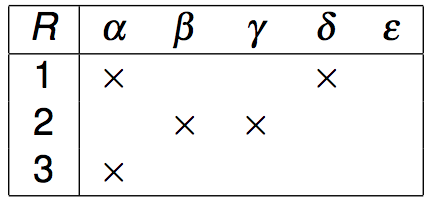
\includegraphics[scale=0.5]{images/1/RelationTable}
\end{center}

Tedy je-li $\langle x, y \rangle \in R$, je v průsečíku řádku $x$ a sloupce $y$ symbol $\times$, jinak tam není nic.

\subsubsection{Maticí}
Matice typu $m \times n$ je obdélníkové schéma o $m$ řádcích a $n$ sloupcích, ve kterém se na každém místě odpovídajícím nějakému řádku a nějakému sloupci nachází nějaká (nejčastěji číselná) hodnota. Označme tuto matici $M$, pro každé $i \in \{1, \dots,m\}$ a $j \in \{1,\dots,n\}$  Nechť $R$ je relace mezi množinami $X = \{x_1,\dots,x_m\}$ a $Y = \{y_1, \dots, y_n\}$. Potom relaci $R$ reprezentujeme maticí tak, že pokud:
$$\langle x_i,y_j\rangle \in R \text{ pak } m_{ij} = 1$$
$$\langle x_i,y_j\rangle \not\in R \text{ pak } m_{ij} = 0$$
Tuto matici nazveme \textbf{matice relace} R a značíme ji $M_R$. Matice $M_R$ relace $R = \{ \langle 1, \alpha \rangle, \langle 2, \gamma \rangle, \langle 1, \delta \rangle, \langle 2, \beta \rangle, \langle 3, \alpha \rangle\}$ mezi množinami \\$X = \{1,2,3\}$ a $Y = \{\alpha, \beta, \gamma, \delta, \epsilon\}$ bude vypadat  následovně.

\begin{displaymath}
{\bf M_R} =
\left( \begin{array}{ccccc}
1 & 0 & 0 & 1 & 0 \\
0 & 1 & 1 & 0 & 0 \\
1 & 0 & 0 & 0 & 0 \\
\end{array} \right)
\end{displaymath}

Nevýhodou této metody je její paměťová složitost. Pokud budeme mít matici $1000 \times 1000$, tak musíme v paměti uchovat milión prvků a pokud z nich bude jen 3000 rovno 1 potom zbytek uchováváme zbytečně protože víme, že na ostatních pozicích musí být 0.

Pro binární relace můžeme zavést operace, které odpovídají operacím s relacemi. Mějme binární matice $M,N$ typu $m \times n$ a matici $K$ typu $n \times k$. Definujeme následující operace:
\begin{itemize}
	\item[] $M \vee N = P, \qquad p_{ij} = max\{m_{ij}, n_{ij}\};$
	\item[] $M \wedge N = P, \qquad min\{m_{ij}, n_{ij}\};$
	\item[] $M - N = P, \qquad max\{0, m_{ij} - n_{ij}\};$
	\item[] $M \cdot K = P, \qquad max\{m_{ij} \cdot k_{ij}; I = 1, \dots ,n\};$
	\item[] $M^T, \qquad m^T_{ij} = m_{ji}$
\end{itemize}

\subsubsection{Grafem}
Grafy představují další způsob reprezentace binárních relací, který je názorný. Graf binární relace $R$ na množině $X$ dostaneme tak, že každý prvek $x \in X$ znázorníme v rovině jako kroužek s označením daného prvku. Pokud $\langle x,y \rangle \in R$, nakreslíme z uzlu $x$ do uzlu $y$ orientovanou hranu.

\begin{center}
	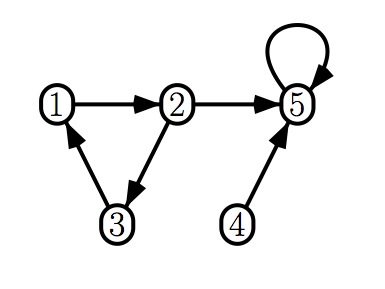
\includegraphics[scale=0.6]{images/1/RelationGraph}
\end{center}

\subsubsection{Seznamem seznamů}
Další způsob reprezentace pro uložení binární relace $R$ na množině $X$ (pro uložení binární relace v paměti počítače) je reprezentace seznamem seznamů. Tuto reprezentaci tvoří hlavní (spojový) seznam, ve kterém jsou uloženy všechny prvky množiny $X$. Z každého prcku $x \in X$ hlavního seznamu vede seznam obsahující právě ty $y \in X$, pro které platí $\langle x, y \rangle \in R$. Mějme relaci $R = \{\langle a, b\rangle,\langle a, d\rangle,\langle c, a\rangle,\langle b, d\rangle\}$ na množině $X = \{a,b,c,d\}$ potom reprezentace seznamem seznamů vypadá následovně.

\begin{center}
	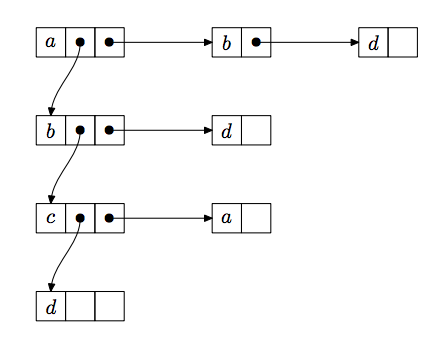
\includegraphics[scale=0.6]{images/1/RelationList}
\end{center}

\subsection{Zobrazení (funkce)}
Zobrazení (funkce) je matematickým protějškem běžně používaného pojmu přiřazení.

\begin{definition}
	Relace R mezi X a Y se nazývá zobrazení (funkce) množiny X do množiny Y, právě když pro každé $x \in X$ existuje právě jedni $y \in Y$ tak že $\langle x, y \rangle \in R$.
\end{definition}

\begin{definition}
	Zobrazení $f : X \rightarrow Y$ se nazývá
	\begin{itemize}
		\item[a)] \textbf{prosté (injektivní)}, právě když pro každé $x_1,x_2 \in X$, pro $x_1 \not= x_2$ plyne $f(x_1) \not= f(x_2)$,
		\item[b)] \textbf{surjektivní} nebo-li zobrazení X \textbf{na} Y, právě když pro každé $y \in Y$ existuje $x \in X$ tak, že  $f(x) = y$,
		\item[c)] \textbf{vzájemně jednoznačné (bijektivní)}, právě když je prosté a na (je tedy injektivní a současně surjektivní).
	\end{itemize}
\end{definition}

\begin{sentence}
	Pro zobrazení $f : X \rightarrow Y, g : Y \rightarrow Z$ platí
	\begin{itemize}
		\item[a)] $f \circ g$ je zobrazení,
		\item[b)] jsou-li f,g injekce, je $f \circ g$ injekce,
		\item[c)] jsou-li f,g surjekce, je $f \circ g$ surjekce.
	\end{itemize}
\end{sentence}

\begin{sentence}
	Nechť $f: A \rightarrow B$ je zobrazení. Inverzní relace $f^{-1}$ je zobrazením $B \rightarrow A$ tehdy a jen tehdy, je-li $f$ bijekce.
\end{sentence}

\begin{result}
	Nechť $f: A \rightarrow B, \ g: B \rightarrow C$ jsou bijekce. Pak
	\begin{itemize}
		\item[a)] $f^{-1} : B \rightarrow A$ je bijekce
		\item[b)] $g^{-1} \circ f^{-1}$ je bijekce C na A a platí $(f \circ g)^{-1} = g^{-1} \circ f^{-1}$.
	\end{itemize}
\end{result}

\begin{definition}
	Nechť $A \not= \emptyset$ je množina. Zobrazení $id_A : A \rightarrow A$ dané předpisem $id_A(x) = x$ pro každé $x \in A$ se nazývá \textbf{identické zobrazení}.
\end{definition}

\begin{definition}
	Nechť $f : A \rightarrow B$ je zobrazení. Pak
	\begin{itemize}
		\item[a)] $f = f \circ id_B = id_A \circ f$
		\item[b)] $f$ je bijekce tehdy a jen tehdy, když existuje zobrazení $g : B \rightarrow A$ tak, že $f \circ g = id_A, g \circ f = id_B$
	\end{itemize}
\end{definition}


\subsubsection{Poznámka k nekonečným množinám}
\begin{definition}
	Množina A se nazývá \textbf{spočetná} , právě když existuje bijekce $f : A \rightarrow \mathbb{N}$. Množina se nazývá \textbf{nespočetná}, právě když je nekonečná a není spočetná.
\end{definition}

\subsection{Binární relace na množině}
Binární relace na množině jsou matematickým protějškem vztahů mezi dvěma prvky množiny například: \uv{$x$ je menší než $y$}. Speciálními relacemi jsou \textbf{prázdná relace $\emptyset$, relace identity} $\omega_X = \{ \langle x, x \rangle \ | \ x \in X \}$, a \textbf{kartézský čtverec} $\tau_X = X \times X$.

\begin{definition}
Nechť $R$ je binární relace na $X$. Řekněme že $R$ je
\begin{itemize}
	\item \textbf{reflexivní}, pokud pro každé $x \in X$ platí $\langle x, x \rangle \in R$
	\item \textbf{symetrická}, pokud pro každé $x,y \in X$ platí $\langle x, y \rangle \in R \Rightarrow \langle y, x \rangle \in R$
	\item \textbf{antisymetrická}, pokud pro každé $x,y \in X$ platí \\$(\langle x, y \rangle \in R \wedge \langle y, x \rangle \in R) \Rightarrow x = y$
	\item \textbf{tranzitivní}, pokud pro každé $x,y,z \in X$ platí \\$(\langle x, y \rangle \in R \wedge \langle y, z \rangle \in R) \Rightarrow \langle x, z \rangle \in R$
	\item \textbf{irreflexivní}, pokud pro každé $x \in X$ platí $\langle x,x \rangle \not\in R$
	\item \textbf{asymetrická}, pokud pro každé $x,y \in X$ platí $\langle x, y \rangle \in R \Rightarrow \langle y, x \rangle \not\in R$
	\item \textbf{úplná}, pokud pro každé $x,y \in X$ platí $\langle x, y \rangle \in R \vee \langle y, x \rangle \in R$
\end{itemize}
\end{definition}

Relace $R$ je \textbf{(relace) ekvivalence}, jestliže je reflexivní, symetrická, a tranzitivní. Relace $R$ je \textbf{(relace) uspořádání}, jestliže je reflexivní, anti\-symetrická a tranzitivní.

\paragraph{Reflexivita} relace $R$ vyjadřuje, že každý prvek $x \in X$ je v relace \uv{sám se sebou}. V matici takovou relaci poznáme že má na diagonále samé 1, v orientovaném grafu je u každého uzlu smyčka.

\paragraph{Symetrie} relace $R$ vyjadřuje, že $\langle x, y \rangle \in R$ právě když  $\langle y, x \rangle \in R$ Tedy relace $R$ je symetrická pokud pro $\forall x,y \in X$ máme buď současně $\langle x, y \rangle \in R$ a  $\langle y, x \rangle \in R$, nebo současně  $\langle x, y \rangle \not\in R$ a  $\langle y, x \rangle \not\in R$. Symetrickou relaci v matici $M_R$ poznáme tak, že je symetrická podle hlavní podle hlavní diagonály. V grafu se tato relace pozná tak že pokud vede orientovaná hrana z $x$ do $y$ pak musí vést i z $y$ do $x$, nebo z $x$ do $y$ nevede žádná hrana.

\paragraph{Antisymetrie} relace $R$ vyjadřuje,že pro každé dav různé prvky $x,y \in X$ neplatí současně $\langle x, y \rangle \in R$ a  $\langle y, x \rangle \in R$. V matici $M_R$ poznáme antisymetrii tak, že dvě různá pole, která jsou souměrná podle diagonály neobsahují dvě jedničky. V grafu se antisymetrie projevuje tak, že meze dvěma různými vrcholy $x,y$ je buď jedna hrana nebo žádná.

\paragraph{Tranzitivita} relace $R$ vyjadřuje, že pro pokud $\langle x, y \rangle \in R$ a pokud $\langle y, z \rangle \in R$, pak také $\langle y, z \rangle \in R$. V grafu je tranzitivita projevuje tak, že pokud vede hrana z $x$ do $y$ a zároveň z $y$ do $z$ potom také $x$ do $z$.

\paragraph{Irreflexivita} relace $R$  vyjadřuje, že žádný prvek $x \in X$ není v relaci \uv{sám se sebou}.
\paragraph{Asymetrie} relace $R$  vyjadřuje, že do $R$ nepadnou $\langle x, y \rangle$ a  $\langle y, x \rangle$ současně.
\paragraph{Úplnost} relace $R$  vyjadřuje, že aspoň jedna z dvojic $\langle x, y \rangle$, $\langle y, x \rangle$ padne do $R$.

\subsection{Uzávěry relací}
Ke každé binární relaci můžeme stanovit její reflexivní, symetrický a tranzitivní uzávěr, to je nejmenší reflexivní, symetrickou a tranzitivní relaci na dané množině, která obsahuje výchozí relaci.

\begin{sentence}
	Nechť R je binární relace na X. Pak
	\begin{itemize}
		\item Ref(R) = $R \cup \omega_X$
		\item Sym(R) = $R \cup R^{-1}$
		\item Tra(R) = $\bigcup^\infty_{n=1} R^n$, kde $R^1 = R$ a $R^n = R \circ R^{n-1}$
	\end{itemize}
\end{sentence}

\subsection{Ekvivalence}
Je binární relace, kterou lze interpretovat jako matematický protějšek nerozlišitelnosti. Pro ekvivalenci $E$ na množině $X$ definujeme pro každý $x \in X$ množinu $[x]_E = \{ y \in X \ | \ \langle x, y \rangle \in E\} $
, kterou nazýváme \textbf{třída ekvivalence prvku} x. Zřejmě $[x]_E$ obsahuje právě ty prvky z $X$, které nelze od $x$ rozlišit ekvivalencí $E$.

\subsection{Rozklad}
Rozklad na množině je matematický protějšek shluků nerozlišitelných prvků. Rozklad na $X$ je \textbf{disjuktní pokrytí} $X$.

\begin{definition}
	Nechť $X \not= \emptyset$. Systém množin $\sqcap \subseteq 2^X$ splňující
	\begin{enumerate}
		\item $Y \not= \emptyset$ pro každou $Y \in \sqcap$,
		\item pro každé $Y_1,Y_2 \in \sqcap$ platí: pokud $Y_1 \cap Y_1 \not= \emptyset$, pak $Y_1 = Y_2$,
		\item $\bigcup\sqcap = X$,
	\end{enumerate}
	se nazývá \textbf{rozklad na množině} X. Množiny $Y \in \sqcap$ nazýváme \textbf{třídy rozkladu} $\sqcap$. Pro prvek $x \in X$ označíme $[x]_\sqcap$ tu třídu rozkladu $\sqcap$, která obsahuje x.
\end{definition}
Na množině $X$ existuji dva mezní rozklady.Prvním z nic je rozklad $\sqcap$, kde $[x]_\sqcap = \{x\}$ pro každé $x \in X$, tj všechny třídy rozkladu $\sqcap$ jsou jednoprvkové. Druhým mezním případem je rozklad $\sqcap = \{X\}$, tj. $\sqcap$ obsahuje jedinou třídu, která je rovna celé $X$, tedy $[x]_\sqcap = X$ pro každé $x \in X$.

\begin{sentence}
	Nechť $\sqcap$ je rozklad na X. Pak binární relace $E_\sqcap$ na X definovaná $\langle x,y \rangle \in E_\sqcap$, právě když $[x]_\sqcap = [y]_\sqcap$ je ekvivalence.
\end{sentence}

Kromě ekvivalencí a rozkladů existují další přirozené pohledy na to \uv{jak zjednodušit nazírání} na výchozí množinu. Jedním z nich je \textbf{surjektivní zobrazení}. Pokud je zobrazení $f : X \rightarrow Y$ surjektivní, pak lez chápat obraz $f(x)$ prvku $x$ jako vyjádření \uv{prvek $x$ nahradíme prvkem $f(x)$}. Ukážeme, že surjektivní zobrazení a ekvivalence mají zvláštní vztah. Pro zobrazení $f : X \rightarrow Y$ definujeme binární relaci $E_f$ na $X$ předpisem $$\langle x , y \rangle \in E_f \qquad \text{právě když} \qquad f(x) = f(y)$$
Zřejmě $E_f$ je ekvivalence, tzv. \textbf{ekvivalence indukovaná zobrazením} $f$.

\subsection{Uspořádání}
Uspořádání je v informatice zcela zásadní ačkoliv si to někdy neuvědomujeme, Mezi základní každého informatika patří znalost problému třídění a typických třídicích algoritmů. Problém třídění jako takový však de facto nemá smysl uvažovat pokud bychom na množině klíčů, podle kterých třídíme, nezavedli nějakou smysluplnou relaci uspořádání -- obvykle ji však chápeme jako \uv{určenou daným kontextem} a explicitně ji nezdůrazňujeme. Uspořádání množin může výrazně zvýšit efektivitu některých algoritmů, například vyhledávání.

\begin{definition}
	Reflexivní, antisymetrická a tranzitivní binární relace R na X se nazývá \textbf{uspořádání}. Úplné uspořádání se nazývá \textbf{lineární uspořádání} neboli \textbf{řetězec}. Pokud je R uspořádání na X, pak se $\langle X, R \rangle$ nazývá \textbf{upořádáná množina}.
\end{definition}

Relace uspořádání na $X$ obvykle značíme $\leq$ v souladu s intuitivním chápáním uspořádání a místo $\langle x ,y \rangle \in \ \leq$. Zdůrazněme ale, že označení $\leq$ v tuto chvíli nemá (obecně) nic společného se srovnáváním čísel, na které jsme zvyklí. Uspořádání pořád ještě není formálním protějškem \uv{upořádání} na které jsme zvyklí při porovnávání čísel. Je-li $\langle X, \leq \rangle$ uspořádaná množina, pak mohou  existovat $x,y \in X$ ,pro které neplatí $x \leq y$ ani $y \leq x$ (definice to nevylučuje). V tom případě říkáme, že prvky jsou \textbf{nesrovnatelné} což někdy značíme $x\ \| \ y$. V opačném případě prvky nazýváme \textbf{srovnatelné}. Je-li $\leq$ lineární uspořádání na $X$, pak je $\leq$ úplná relace, což znamená, že každé prvky jsou srovnatelné. Lineární uspořádání lze tedy chápat jako matematický protějšek \uv{tradičního srovnávání čísel}. Každá relace identity $\omega_X$ je uspořádání které nazýváme \textbf{antiřetězec}

\begin{sentence}
	Princip duality. Nechť $\leq$ je uspořádání na $X$. Pak $\leq^{-1}$ je uspořádání na $X$, které označujeme $\geq$.
\end{sentence}

Konečné uspořádání $\leq$ na $X$ je relace, mžeme ji tedy reprezentovat binární maticí nebo příslušným orientovaným grafem. Díky speciálním vlastnostem konečných uspořádání je však můžeme znázorňovat mnohem přehledněji pomocí speciálních diagramů. Ke každému uspořádání $\leq$ na $X$ lze uvažovat odvozenou relaci $\prec$ definovanou předpisem
$$x \prec y, \text{ právě když } x \leq y \text{ a } \forall z \in X \text{ platí: }$$
$$\text{pokud} y \leq z \leq y, \text{ pak } z \in \{ x, y\}$$



Relaci $\prec$ nazýváme pokrytí příslušné $\leq$ , a výraz $x \prec y$ čteme \uv{x je pokryt y} nebo \uv{x pokrývá y}. Na relaci pokrytí je založena jedna z metod jak znázornit konečnou uspořádanou množinu, tak zvané \textbf{Hasseovy diagramy} uspořádaných množin.

\begin{center}
	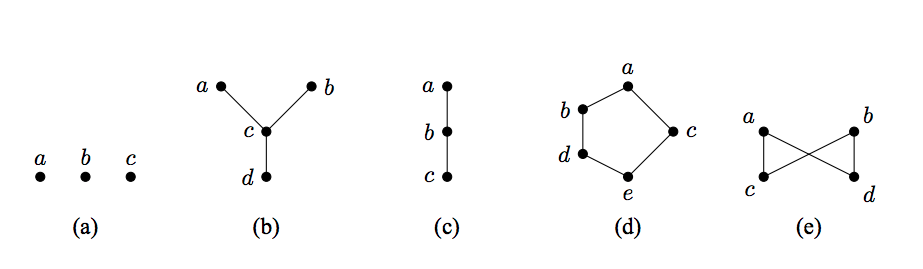
\includegraphics[scale=0.9]{images/1/HasseDiagrams}
\end{center}

\begin{definition}
	Nechť $\langle X, \leq \rangle$ je uspořádaná množina. Prvek $x \in X$ se nazývá
	\begin{itemize}
		\item \textbf{minimální}, jestliže $\forall y \in X$ platí: pokud $y \leq x$, pak $x = y$,
		\item \textbf{nejmenší}, jestliže $x \leq y$ pro každá $y \in X$,
		\item \textbf{maximální}, jestliže $\forall y \in X$ platí: pokud $y \geq x$ pak $x = y$,
		\item \textbf{nejmenší}, jestliže $x \geq y$ pro každý $y \in X$.
	\end{itemize}
\end{definition}

\begin{sentence}
	Nechť $\langle X, \leq \rangle$ je uspořádaná množina. Pak platí
	\begin{enumerate}
		\item v $\langle X, \leq \rangle$ existuje nejvýše jeden největší a nejvýše jeden nejmenší prvek;
		\item je-li $x \in X$ největší (nejmenší) prvek, pak je také maximální (minimální);
		\item pokud je $\leq$ lineární uspořádání, pak je $x \in X$ největší (nejmenší) prvek, právě když je maximální (minimální).
	\end{enumerate}
\end{sentence}

\begin{definition}
	Nechť $\langle X, \leq \rangle$ je uspořádaná množina a nechť $Y \subseteq X$. Definujeme množiny
	$$L(Y) = \{ x \in X \ | \ x \leq y \text{ platí pro každé } y \in Y\}$$
	$$U(Y) =  \{ x \in X \ | \ x \geq y \text{ platí pro každé } y \in Y\}$$
	L(Y) se nazývá \textbf{dolní kužel množiny} Y v  $\langle X, \leq \rangle$. U(Y) se nazývá \textbf{horní kužel množiny} Y v  $\langle X, \leq \rangle$.
\end{definition}

Jinými slovy dolní kužel množiny $Y$ v  $\langle X, \leq \rangle$ obsahuje tedy právě ty prvky z $X$, které jsou menší nebo rovny všem prvkům obsaženým v $Y$, analogicky pro horní kužel.

\begin{definition}
	Nechť  $\langle X, \leq \rangle$ je uspořádaná množina a nechť $Y \subseteq X$. Pokud má $L(Y)$ největší prvek, pak se nazývá \textbf{infimum} Y a označuje se $inf(Y)$. Pokud má $U(Y)$ nejmenší prvek, pak se nazývá \textbf{supremum} Y a označuje se $sup(Y)$.
\end{definition}

\begin{definition}
	Nechť  $\langle X, \leq \rangle$ je uspořádaná množina. Pokud pro každé $x,y \in X$ existuje $inf(x,y)$, pak  $\langle X, \leq \rangle$ nazveme \textbf{průsekový polosvaz}. Pokud pro každé $x,y \in X$ existuje $sup(x,y)$ pak  $\langle X, \leq \rangle$ nazveme \textbf{spojový polosvaz}. Je-li  $\langle X, \leq \rangle$ průsekový i spojový polosvaz, pak  $\langle X, \leq \rangle$ nazveme \textbf{svaz}.
\end{definition}

\newpage
\textbf{Vektorové prostory, lineární závislost a nezávislost, báze a dimenze vektorového prostoru. Eukleidovské vektorové
prostory. Matice, determinanty: vlastnosti, operace s nimi. Řešení soustav lineárních rovnic. Algebraické
struktury: grupa, okruh, obor integrity, těleso. Svazy: modulární, distributivní, komplementární.}

\section{Algebraické struktury}
\subsection{Grupoid}
\begin{definition}
	Nechť $A \not= \emptyset$. Binární operací na množině A nazveme každé zobrazení $f : A \times A \rightarrow A$.
\end{definition}

\begin{example}
	Nechť $\mathbb{Z}$ je množina všech celých čísel, + přiřadí každé dvojici čísel $a,b \in \mathbb{Z}$ číslo $a + b \in \mathbb{Z}$. Je tedy binární operace.
\end{example}

\begin{definition}
	Nechť $A \not= \emptyset$ a $\circ$ je binární operace na A. Dvojici $\mathscr{A} = (A, \circ)$ budeme nazývat grupoid. Jeli operace $\circ$ asociativní, tj. jestliže $\forall a,b,c \in A$ platí $a \circ (b \circ c) = (a \circ b) \circ c$, nazývá se grupoid $(A, \circ)$ pologrupa. Operace $\circ$ se nazývá komutativní jestliže $a \circ b = b \circ a$ pro každé $a,b \in A$.
\end{definition}

Budeme-li operaci v grupoidu zapisovat symbolem +, nazýváme grupoid $(A, +)$ \textbf{aditivní}, budeme-li operaci zapisovat $\circ$ (nebo vynechávat), nazývá se grupoid $(A, \circ)$ \textbf{multiplikativní}.

\begin{definition}
	Jestliže v grupoidu $(A, \circ)$ existuje prvek $e$ takový, že $a \circ e = e \circ a = a$ pro každé $a \in A$, nazývá se e \textbf{jednotkou} $(A, \circ)$. Jestliže v A existuje prvek n takový, že $a \circ n = n \circ a = n$, nazývá se n \textbf{nula} grupoidu $(A, \circ)$.
\end{definition}

\begin{definition}
	Nechť $\mathscr{A} = (A, \circ)$ je grupoid, nechť $\emptyset \not= B \subseteq A$.Jestliže $\forall a,b \in B$ platí $a \circ b \in B$, nazývá se $(B, \circ)$ \textbf{podgrupoid} grupoidu $\mathscr{A}$.
\end{definition}

\subsection{Grupa}
\begin{definition}
	Nechť $(A, \circ)$ je pologrupa. Jestliže pro každé dva prvky $a,b \in A$ existují $x,y \in A$ tak, že platí  $a \circ x = b, y \circ a = b$, pak se $(A, \circ)$ se nazývá \textbf{grupa}.
\end{definition}

Další možností jak definovat to, že je grupoid $\mathscr{G}$ grupa říká následující definice.
\begin{definition}
	 $\mathscr{G} = (G, \circ)$  nazveme grupou pokud platí
	\begin{enumerate}
		\item $\forall a,b, \in G : a \circ b \in G$ (uzavřenost)
		\item $\forall a,b,c \in G : (a \circ b) \circ c = a \circ (b \circ c)$ (asociativita)
		\item $\exists e \in G \quad \forall a \in G : a \circ e = e \circ a = a$ (jednotkový prvek)
		\item $\forall a \in G \quad \exists a^{-1} \in G : a \circ a^{-1} = a^{-1} \circ a = e$ (inverzní prvek)
	\end{enumerate}
	Grupa se nazývá \textbf{abelovská} právě když platí komutativita: $$\forall a,b, \in G : a \circ b = b \circ a$$
\end{definition}

\begin{definition}
	Nechť $\mathscr{G} = (G, \circ)$ je grupa. Podgrupoid $(A, \circ)$ grupoidu $(G, \circ)$ se nazývá \textbf{podgrupa grupy} $\mathscr{G}$, je-li $(A, \circ)$ grupou.
\end{definition}

\begin{example}
	Grupa $(\mathbb{Z}, +)$ je podgrupou grupy $(\mathbb{R}, +)$ všech reálných čísel.
\end{example}

\subsection{Okruh}
\begin{definition}
	\textbf{Okruhem} nazveme trojici $\mathscr{R} = (R, + , \cdot)$ takovou, že $R \not= \emptyset$ je množina, + a $\cdot$ jsou binární operace na R a
	\begin{enumerate}
		\item $(R, +)$ je abelovská grupa (0 její jednotka)
		\item $(R, \cdot)$ je pologrupa
		\item Platí \textbf{distributivní zákony}, tj. pro každé $a,b,c \in R$ platí $$a \cdot (b + c) = a \cdot b + a \cdot +\ c, \qquad (b + c) \cdot a = b \cdot a + c \cdot a$$
	\end{enumerate}
	Okruh $\mathscr{R}$ se nazývá \textbf{komutativní}, jestliže $ a \cdot b = b \cdot a$ pro každé $a,b \in R$. Okruh $\mathscr{R}$ se nazývá \textbf{unitární}, má-li pologrupa $(R \setminus \{0\}, \cdot)$ jednotku. Je-li $\mathscr{R}$ unitární, budeme jeho jednotku označovat 1. Prvek 0 (jednotka $(R, +)$) se nazývá \textbf{nulou okruhu} $\mathscr{R}$.
\end{definition}

\begin{example}
	Komutativní unitární okruhy jsou například: okruh celých čísel $(\mathbb{Z}, + , \cdot)$, okruh reálných čísel $(\mathbb{R}, + , \cdot)$, okruh komplexních čísel $(\mathbb{C}, + , \cdot)$ a okruh racionálních čísel $(\mathbb{Q}, + , \cdot)$.
\end{example}

\begin{definition}
	Prvek a okruhu $\mathscr{R} = (R,+,\cdot)$ se nazývá \textbf{dělitel nuly}, jestliže $a \not= 0$ existuje $b \not= 0, b \in R$ tak, že $a \cdot b = 0$.
\end{definition}

\subsection{Obor integrity}
\begin{definition}
	Okruh $\mathscr{R} = (R,+,\cdot)$ se nazývá \textbf{obor integrity}, je-li komutativní, unitární a neobsahuje dělitele nuly.
\end{definition}

\begin{example}
	Každý z okruhů $(\mathbb{Z}, + , \cdot)$, $(\mathbb{R}, + , \cdot)$,  $(\mathbb{C}, + , \cdot)$, $(\mathbb{Q}, + , \cdot)$ je obor integrity.
\end{example}


\subsection{Těleso}
\begin{definition}
	Okruh $\mathscr{R} = (R,+,\cdot)$ se nazývá \textbf{těleso}, je-li množina jeho nenulových prvků grupou vzhledem k operaci $\cdot$. Těleso $\mathscr{R}$ se nazývá \textbf{komutativní}, je-li $(R \setminus \{0\}, \cdot)$ abelovská grupa.
\end{definition}

\begin{example}
	Okruhy  $(\mathbb{R}, + , \cdot)$,  $(\mathbb{C}, + , \cdot)$, $(\mathbb{Q}, + , \cdot)$ jsou komutativní tělesa. Okruh $(\mathbb{Z}, + , \cdot)$ není těleso.
\end{example}

\begin{sentence}
	Každé komutativní těleso je obor integrity.
\end{sentence}

\begin{definition}
	Je-li  $\mathscr{R} = (R,+,\cdot)$ okruh, $A \subseteq R$ taková že  $(A,+,\cdot)$ je opět okruh, pak se    $(A,+,\cdot)$ nazývá \textbf{podokruh okruhu} $\mathscr{R}$. Je-li  $\mathscr{R} = (R,+,\cdot)$ těleso, $A \subseteq R$ taková že  $(A,+,\cdot)$ je opět těleso, pak se $(A,+,\cdot)$ nazývá \textbf{podtěleso tělesa} $\mathscr{R}$. Každé podtěleso tělesa $\mathscr{C} = (C,+,\cdot)$  komplexních čísel nazveme \textbf{číselné těleso}. Každý podokruh okruhu  $\mathscr{C}$ nazveme \textbf{číselný okruh}.
\end{definition}

\begin{example}
	 $ \mathscr{R} = (\mathbb{R}, + , \cdot)$,  $\mathscr{C} = (\mathbb{C}, + , \cdot)$, $ \mathscr{Q} = (\mathbb{Q}, + , \cdot)$ jsou číselná tělesa. $\mathscr{Z} = (\mathbb{Z}, + , \cdot)$ je číselný okruh, který není tělesem.
\end{example}

\section{Vektorové prostory}
\begin{definition}
	Nechť $A \not= \emptyset \not= B$ jsou množiny. Zobrazení $\circ : A \times B \rightarrow B$ nazveme \textbf{levá vnější operace nad množinami} A,B (v tomto pořadí). Jsou-li $a \in A, b \in B$, pak prvek $\circ(a,b)$ budeme zapisovat $a \circ b$.
\end{definition}

\begin{definition}
	Nechť $(V, +)$ je abelovská grupa, nechť T je číselné těleso, nechť $\circ : T \times V \rightarrow V$ je levá vnější operace nad T,V. Pak čtveřici $\mathscr{V} = (V, +, T, \circ)$ nazveme \textbf{vektorový prostor nad} T, platí-li $\forall u,v \in V, \forall c,d, \in T$
	\begin{enumerate}
		\item $c \circ (u + v) = c \circ u + \circ v$
		\item $(c + d) \circ u = c \circ u + d \circ u$
		\item $(c \cdot d) \circ u = c \circ (d \circ u)$
		\item $1 \circ u = u$
	\end{enumerate}
	Prvky v V budeme nazývat \textbf{vektory}, čísla z tělesa T \textbf{skaláry}. Množinu V nazveme \textbf{pole} vektorového prostoru $\mathscr{V}$.
\end{definition}

\begin{definition}
	Nechť  $\mathscr{V}$ je vektorový prostor nad tělesem T, nechť $v,u_1,\dots,u_k \in V$. Řekneme, že vektor v je \textbf{lineární kombinací vektorů}  $v,u_1,\dots,u_k$, jestliže existují čísla $c_1, \dots, c_k \in T$ tak, že $$v = c_1 \cdot u_1 + \dots + c_k \cdot u_k$$
\end{definition}
\paragraph{Poznámka.} Symbolem \textbf{o} budeme označovat tzv. \textbf{nulový vektor}, což je jednotka grupy $(V, +)$. Použitím podmínky 2. dostaneme $\forall u \in V:$ $$0 \cdot u = (c + (-c)) \cdot u = c \cdot u + (-c \cdot u) = o$$
Tedy nulový vektor je lineární kombinací libovolných vektorů z $V: $ je-li $u_1,\dots,u_k \in V$ pak $$0 \cdot u_1 + \dots + 0 \cdot u_k = o$$


\begin{definition}
	Vektory $u_1, \dots, u_k$ z vektorového prostoru $\mathscr{V}$ se nazývají \textbf{lineárně nezávislé}, jestliže existují čísla $c_1, \dots, c_k \in T$, která nejsou všechna rovna nule tak, že nulový vektor \textbf{o} je roven netriviální lineární kombinaci vektorů $u_1, \dots, u_k$, tj. $$o = c_1 \cdot u_1 + \dots + c_k \cdot u_k,$$
	kde aspoň jedno $c_i \not= 0$. Jestliže vektory $u_1, \dots, u_k$ nejsou lineárně závislé, nazývají se \textbf{lineárně nezávislé}.
\end{definition}

\paragraph{Poznámka.} Zřejmě vektory  $u_1, \dots, u_k \in \mathscr{V}$ jsou lineárně nezávislé, právě když $$o = c_1 \cdot u_1 +  \dots + c_k \cdot u_k \quad \Rightarrow \quad c_1 = c_2 = \dots = c_k = 0$$

\begin{sentence}
	Jsou-li mezi vektory  $u_1, \dots, u_k \in \mathscr{V}$  některé lineárně závislé, pak jsou  $u_1, \dots, u_k$ lineárně závislé.
\end{sentence}

\begin{sentence}
	Je-li mezi vektory  $u_1, \dots, u_k$  vektor nulový \textbf{o}, pak jsou $u_1, \dots, u_k$ lineárně závislé.
\end{sentence}

\begin{sentence}
	Nechť $u_1, \dots, u_k \in \mathscr{V}$. Pak  $u_1, \dots, u_k$ jsou lineárně závislé, právě když je aspoň jeden z nich lineární kombinací ostatních vektorů.
\end{sentence}

\begin{definition}
	Nechť  $\mathscr{V} = (V, +, T, \circ)$  je vektorový prostor nad tělesem T, nechť $\emptyset \not= W \subseteq V$. Pak  $\mathscr{W} = (W, +, T, \circ)$ nazveme \textbf{podprostor vektorového prostoru} $\mathscr{V}$, jestliže
	\begin{enumerate}
		\item $\forall u,c \in W$ je $u + v \in W$
		\item $\forall u \in W, \forall c \in T$ je $c \cdot u \in W$.
	\end{enumerate}
\end{definition}


\begin{definition}
	nechť M je podmnožina vektorového prostoru $\mathscr{V}$. \textbf{Lineárním obalem množiny M ve} $\mathscr{V}$ rozumíme množinu všech lineárních kombinací vektorů z M.
\end{definition}

\begin{definition}
	Nechť  $\mathscr{V}$ je vektorový prostor, $m \not= \emptyset$ jeho podmnožina. Je-li $[M] =\mathscr{V}$, nazývá se M množina generátorů  $\mathscr{V}$.
\end{definition}

\begin{definition}
	Řekněme, že vektorový prostor $\mathscr{V}$ je konečné dimenze, má-li aspoň jednu konečnou množinu generátorů.
\end{definition}

\begin{definition}
	Bází vektorového prostoru $\mathscr{V}$ konečné dimenze rozumíme libovolnou lineárně nezávislou konečnou množinu $\{u_1, \dots, u_n\}$ jeho generátorů.
\end{definition}

\begin{sentence}
	Nechť $M = \{u_1, \dots, u_n\}$ je bází $\mathscr{V}$. Pak každý vektor $v \in \mathscr{V}$ lze jediným způsobem vyjádřit jako lineární kombinaci vektorů $u_1, \dots, u_n$.
\end{sentence}

\begin{example}
	Příklad báze vektorového prostoru $e_1 = (1,0,0,0), e_2 = (0,1,0,0), e_3 = (0,0,1,0), e_4 = (0,0,0,1)$
\end{example}

\begin{definition}
	Je-li $\mathscr{V} \not= \{o\}$  vektorový prostor konečné dimenze, pak počet prvků jeho libovolné báze nazýváme dimenze $\mathscr{V}$ a značíme $dim\mathscr{V}$, Je-li $\mathscr{V} = \{o\}$, položíme dim$\mathscr{V} = 0$.
\end{definition}

\section{Eukleidovské vektorové prostory}
Ve vektorovém prostoru nad tělesem $T$ můžeme vektory sčítat, odčítat a násobit skaláry z tělesa $T$ (levá vnější operace). Nemáme však zaveden pojem délky vektoru, úhlu mezi vektory apod. Zavedeme proto další pojem.

\begin{definition}
	Nechť $\mathscr{V} = (V, +, \mathbb{R}, \cdot)$ je vektorový prostor nad tělesem reálných čísel $\mathbb{R}$. \textbf{Skalárním součinem} $\circ$ nazveme zobrazení $V \times V$ do tělesa $\mathbb{R}$, které má tyto vlastnosti:
	\begin{enumerate}
		\item $\forall u,v \in V, u \circ v = v \circ u$
		\item $\forall u \in V, u \not= o, u \circ o > 0$
		\item $\forall u,v,w \in V, (u + v) \circ w = u \circ w + v \circ w$
		\item $\forall u,v \in V, \forall c \in \mathbb{R}, (c \cdot u) \circ v = c \cdot (u \circ v)$.
	\end{enumerate}
\end{definition}

\begin{example}
	Je-li $\mathscr{V} = (\mathbb{R}^n, +, \mathbb{R}, \cdot)$ aritmeticky (n-dimenzionální) vektorový prostor nad $\mathbb{R}, x = (x_1,x_2, \dots, x_n), y = (y_1,y_2, \dots, y_n)$, pak $x \circ y = \sum^n_{i=1} x_i \cdot y_i$ definuje skalární součin $\circ$.
\end{example}

\begin{definition}
	Nechť $\mathscr{V} = (V, + \mathbb{R}, \cdot)$ je vektorový prostor nad tělesem reálných čísel, ve kterém je definován skalární součin. Pak se $\mathscr{V}$ nazývá \textbf{Eukleidovský vektorový prostor}
\end{definition}

\begin{definition}
	Nechť $\mathscr{V}$ je Eukleidovský vektorový prostor, nechť $u \in V$. Číslo $\| u \| = \sqrt{u \circ u}$ nazveme délka vektoru u.
\end{definition}

\begin{definition}
	Nechť $\mathscr{V}$ je Eukleidovský vektorový prostor, $u,v \in V$. Pak
	\begin{itemize}
		\item[a)] $\forall c \in \mathbb{R}$ je $\| c \cdot u \| = |c| \cdot \| u \|$
		\item[b)] $\| o \|$ a pro $u \not= o$ je $\| u \| > 0$
		\item[c)] $|u \circ v| \leq \| u \| \cdot \| v \|$ (Schwarzova nerovnost)
	\end{itemize}
\end{definition}

\begin{definition}
	Nechť $\mathscr{V}$ je Eukleidovský vektorový prostor, $u,v \in V$, $u \not= o \not= v$. Úhlem $\varphi$ vektorů u,v nazveme číslo $$\varphi = arccos \frac{u \circ v}{\| u \| \cdot \| v \|}$$
\end{definition}
Platí tedy $cos \varphi = \frac{u \circ v}{\| u \| \cdot \| v \|}$, kde $0 < \varphi < \pi$

\begin{definition}
	Vektory u,v nazveme ortogonální (kolmé). ozn. $u \bot v$, je-li $\varphi = \frac{\pi}{2}$ tj. $cos \varphi = 0$, tj. $u \circ v = 0$.
\end{definition}

\begin{definition}
	Vektory $u_1, \dots, u_m$ jsou vzájemně ortogonální, platí-li $u_i \bot u_j$ pro každé $i \not= j$.
\end{definition}

\begin{sentence}
	Nenulové vzájemně ortogonální vektory $u_1, \dots, u_m$ jsou lineárně nezávislé.
\end{sentence}

\begin{definition}
	Jsou-li  $u_1, \dots, u_m$ vzájemně ortogonální vektory, přičemž $\{ u_1, \dots, u_m\}$ generuje celý prostor $\mathscr{V}$, pak je to báze $\mathscr{V}$ (tzv. ortogonální báze).
\end{definition}

\section{Matice}
\begin{definition}
	Nechť T je číselné těleso, m,n jsou čísla přirozená a nechť $a_{ij} \in T$  pro $i = 1, \dots, m, j = 1, \dots n.$ Dvojindexované schéma
\begin{displaymath}
{\bf A} =
\left( \begin{array}{cccc}
a_{11} & a_{12} & \dots & a_{1n} \\
a_{21} & a_{22} & \dots & a_{2n} \\
\vdots &  &  &  \\
a_{m1} & a_{m2} & \dots & a_{mn} \\
\end{array} \right)
\end{displaymath}
se nazývá matice typu $m \times n$ nad T. Číslo $a_{ij}$ se nazývá prvek matice A z i-tého řádku a j-tého sloupce. Číslo i se nazývá řádkový, číslo j sloupcový index prvku $a_{ij}$.
\end{definition}

\paragraph{Poznámka.} Někdy budeme matice značit následovně: $A = \| a_{ij}\|$.

\begin{definition}
	Matice $A = \|a_{ij}\|$ typu $m \times n$, kde $m = n$ se nazývá čtvercová matice stupně n. Čtvercová matice A se nazývá diagonální pokud pro všechny její prvky. která neleží na hlavní diagonále jsou rovny 0. Diagonální matice se nazývá skalární, jestliže všechny její prvky na hlavní diagonále jsou si rovny. Skalární matice se nazývá jednotková stupně n, jsou-li všechny její prvky na hlavní diagonále rovny 1 (budeme ji označovat $E_n$). Matici N typu $m \times n$ nazveme nulová matice jestliže jsou všechny její prvky rovny 0.
\end{definition}

\paragraph{Označení.} Symbolem $\mathscr{M}_{m \times n}(T)$ resp. $\mathscr{M}_{n}(T)$ označíme množinu všech matic typu $m \times n$ resp. všech čtvercových matic stupně $n$ nad tělesem $T$.

\begin{definition}
	Dvě matice $A,B$ z $\mathscr{M}_{m \times n}(T)$ jsou si rovny, jestliže $a_{ij} = b_{ij}$ pro každé  $i = 1, \dots, m, j = 1, \dots n.$
\end{definition}

\begin{definition}
	Mějme matice $A,B \in \mathscr{M}_{m \times n}(T)$. Součtem matice $A$ a $B$ rozumíme matici $A + B = \|c_{ij}\|$, kde $ \|c_{ij}\| =  a_{ij} + b_{ij}$ pro každé $i = 1, \dots, m, j = 1, \dots n.$
\end{definition}

\begin{sentence}
	Množina $\mathscr{M}_{m \times n}(T)$ spolu se zavedenou operací sčítání matic tvoří abelovskou grupu.
\end{sentence}
\begin{definition}
	Nechť T je číselné těleso, $A \in \mathscr{M}_{m \times n}(T)$. Prvky z T budeme nazývat skaláry. zavedeme levou vnější operaci $\cdot : T \times  \mathscr{M}_{m \times n}(T) \rightarrow \mathscr{M}_{m \times n}(T)$ takto: $c \in T, \ A= \| a_{ij} \| \ pak \ cA = \|c \cdot a_{ij} \|$ je tzv. násobení matice skalárem.
\end{definition}

\begin{definition}
	Nechť $A= \| a_{ij} \|$ je matice typu $m \times n$. Matici transponovanou k matici A nazýváme matici $A^T = \| a_{ji} \|$ typu $n \times m$ která vznikne z A vzájemnou výměnou řádků a sloupců (tj. otočením A podle hlavní diagonály).
\end{definition}

\begin{definition}
	Nechť $A= \| a_{ij} \|$ je matice typu $m \times n$ a nechť $B= \| b_{jk} \|$ je matice typu $n \times p$  nad tělesem T. Součinem matic A a B (v tomto pořadí) nazveme matici $AB =  \| c_{ik} \|$ typu $m \times p$ pro jejíchž prvky platí: $$c_{ik} = a_{i1}b_{1k} + a_{i2}b_{2k} + \dots + a_{in}b_{nk} = \sum^n_{j=1} a_{ij}b_{jk}$$
	pro každé $i = 1, \dots, m, k = 1, \dots p.$
\end{definition}

\begin{sentence}
	Násobení matic je asociativní, tj. jestliže $A \in \mathscr{M}_{m \times n}(T), B \in \mathscr{M}_{n \times p}(T), C \in \mathscr{M}_{p \times r}(T)$, pak $$(AB)C = A(BC).$$
\end{sentence}

\begin{sentence}
	Nechť T je těleso $n \in \mathbb{N}$. Pak $ \mathscr{M}_{n}(T) = (\mathscr{M}_{n}(T) ,+,\cdot)$ je unitární okruh, jehož jednotkou je jednotková matice. Je-li $n > 1$ pak tento okruh není komutativní a obsahuje dělitele nuly. Je-li $n = 1$ pak $\mathscr{M}_{1}(T)$  je komutativní těleso.
\end{sentence}

\section{Determinanty}

\begin{definition}\end{definition}
\begin{definition}\end{definition}
\begin{definition}\end{definition}
\begin{definition}\end{definition}



% ---------------------------------------------------------------------------------------------------------
% --------------------------------------------- pátý odstavec ---------------------------------------------
% ---------------------------------------------------------------------------------------------------------
\newpage
\textbf{Kombinatorika: pravidlo součtu a součinu, permutace, variace, kombinace, binomická věta, princip inkluze a
exkluze. Popisná statistika: číselné charakteristiky výběrů a grafické metody.}

\section{Kombinatorika}
\subsection{Pravidlo součtu a součinu}
\subsubsection{Pravidlo součtu}
\begin{definition}
	Lze-li úkol A provést m-způsoby a lze-li úkol B provést n-způsoby,
přičemž žádný z m-způsobů provedení úkolu A není totožný s žádným z n-způsobů
provedení úkolu B, pak provést úkol A nebo úkol B lze provést m + n způsoby.
\end{definition}

\subsubsection{Pravidlo součinu}
\begin{definition}
	Lze-li úkol C rozložit na po sobě následující úkoly A a B (tj. provést
C znamená provést nejdřív A a potom B) a lze-li úkol A provést m způsoby a úkol B lze
provést n způsoby, pak lze úkol C provést $m \cdot n $ způsoby.	
\end{definition}

\subsection{Variace}
\subsubsection{bez opakování}
\begin{definition}
	Je dáno n (navzájem různých) objektů a číslo $r \leq n$. Variace r
(objektů) z n (objektů) je libovolný výběr r objektů z daných n objektů, ve kterém záleží na
pořadí vybíraných objektů. Počet takových variací značíme V(n, r).
\end{definition}
\begin{sentence}
	$V(n, r) = n \cdot (n - 1) \cdot \dots \cdot (n - r + 1)$
\end{sentence}
\paragraph{Poznámka.} $V(n, r) = \frac{n!}{(n - r)!} = \frac{n \cdot (n - 1) \cdot \dots \cdot (n - r + 1) \cdot (n - r) \cdot \dots \cdot 1}{(n - r) \cdot \dots \cdot 1} = n \cdot (n - 1) \cdot \dots \cdot (n - r + 1)$

\subsubsection{s opakováním}
\begin{definition}
	Jsou dány objekty n různých typů. Objektů každého typu je neomezeně mnoho a jsou navzájem nerozlišitelné. Variace r (objektů) z n (objektů) s opakováním je libovolný výběr r objektů z daných objektů n typů, ve kterém záleží na pořadí vybíraných objektů. Počet takových variací značíme $\overline{V}(n, r)$.	
\end{definition}
\begin{sentence}
	$\overline{V}(n, r) = n^r$.
\end{sentence}

\subsection{Permutace}
\subsection{bez opakování}
\begin{definition}
	Permutace n (navzájem různých) objektů je libovolné seřazení těchto objektů, tj. seřazení od prvního k n-tému. Počet permutací n objektů budeme značit P(n).
\end{definition}
\begin{sentence}
	$P(n) = V(n, n) = n!$
\end{sentence}

\subsection{s opakováním}
\begin{definition}
	Je dáno n objektů rozdělených do r skupin, které mají po řadě $n_1, \dots,n_r$ objektů, tj. $n_1 + \dots + n_r = n$. Objekty v každé ze skupin jsou navzájem nerozlišitelné. Každé seřazení těchto n objektů se nazývá permutace s opakováním (daným parametry ($n_1, \dots, n_r$)). Počet takových permutací značíme P($n_1, \dots, n_r$).
\end{definition}
\begin{sentence}
	Pro $n_1 + \dots + n_r = n$ je P($n_1, \dots, n_r$)$ = \frac{n!}{n_1! \cdot \dots \cdot n_r!}$.
\end{sentence}

\subsection{Kombinace}
\subsubsection{bez opakování}
\begin{definition}
	Je dáno n (navzájem různých) objektů a číslo $r \leq n$. Kombinace r (objektů) z n (objektů) je libovolný výběr r objektů z daných n objektů, ve kterém nezáleží na pořadí vybíraných objektů. Počet takových kombinací značíme $n \choose r$ (nebo C(n, r)).
\end{definition}
\begin{sentence}
	${n \choose r} = \frac{n!}{(n - r)! \cdot r!}$
\end{sentence}
$$ {n \choose r} = {n \choose n - r} $$
\\ $${n \choose n} = 1 \text{ a } {n \choose 0} = 1 $$
\paragraph{Poznámka.} ${n \choose k} = {n - 1 \choose k - 1} + {n - 1 \choose k}$.

\subsubsection{s opakováním}
\begin{definition}
	Jsou dány objekty n různých typů. Objektů každého typu je neomezeně mnoho a jsou navzájem nerozlišitelné. Kombinace r (objektů) z n (objektů) s opakováním je libovolný výběr r objektů z daných objektů n typů, ve kterém nezáleží na pořadí vybíraných objektů. Počet takových kombinací značíme $\overline{C}(n, r)$.
\end{definition}
\begin{sentence}
	$\overline{C}(n, r) = {n + r - 1 \choose n - 1}$.
\end{sentence}

\subsection{Binomická věta}
\begin{sentence}
Pro reálné číslo $x$ a nezáporné celé $n$ je $$(1 + x)^n = \sum\limits_{k=0}^n {n \choose k} x^k $$
\end{sentence}

\subsection{Princip inkluze a exkluze}
\begin{sentence}
	Pro množiny $A_1, \dots, A_n$ platí $$|A_1 \cup A_2 \cup \dots \cup A_n| = \sum\limits_{\emptyset \neq I \subseteq \{1, 2, \dots , n \}} (-1)^{|I| + 1} |\bigcap_{i \in I} A_i |$$
\end{sentence}
\begin{example}
	V nabídce volitelných předmětů je němčina a angličtina. Němčinu si zvolilo 15, angličtinu 30 a oba jazyky 5 studentů. Kolik studentů si jako volitelný předmět vybralo cizí jazyk (tj. NJ + AJ)? Označme N a A po řadě množiny studentů, kteří si zapsali NJ a AJ. Sečteme-li $|N|$ (počet co si zapsali němčinu) a $|A|$ (počet co si zapsali angličtinu), počítáme dvakrát ty, kteří si zapsali NJ a AJ (těch je $|N \cap A|$. Ty tedy musíme od $|N| + |A|$ odečíst. Počet $|N \cup A|$ těch, kteří si zapsali NJ nebo AJ tedy $$|N \cup A| = |N| + |A| - |N \cap A| = 15 + 30 - 5 = 40$$
\end{example}
\paragraph{Poznámka.} $|A_1 \cup A_2 \cup A_3| = |A_1| + |A_2| + |A_3| - |A_1 \cap A_2| - |A_1 \cap A_3| - |A_2 \cap A_3| + |A_1 \cap A_2 \cap A_3|$

\section{Popisná statistika}
\subsection{Číselné charakteristiky výběrů}
\subsubsection{Výběrový (aritmetický) průměr}


\subsubsection{Medián}
\subsubsection{Výběrový rozptyl}
\subsubsection{Směrodatná odchylka}

\subsection{Grafické metody}



% ---------------------------------------------------------------------------------------------------------
% --------------------------------------------- šestý odstavec ---------------------------------------------
% ---------------------------------------------------------------------------------------------------------
\newpage
\textbf{Náhodné jevy, pravděpodobnostní míra. Podmíněná pravděpodobnost, nezávislost jevů. Náhodná veličina, distribuční
funkce. Příklady rozdělení diskrétních a spojitých náhodných veličin. Náhodné vektory: sdružené a
marginální rozdělení. Bodové odhady. Základy testování hypotéz.}




\end{document}
